\documentclass[12pt,letterpaper]{hmcpset}
\usepackage[margin=1in]{geometry}
\usepackage{graphicx}
\usepackage{enumitem} % enumerate
\newcommand{\vb}{\mathbf}
\usepackage{amsmath}

% example usage of amssymb: $\mathbb{Z}$
% amsmath is loaded.

% info for header block in upper right hand corner
\name{}
\class{Math 19 - \phantom{07}}
\assignment{Homework \#10}
\duedate{11/22/2019}

\begin{document}
\problemlist{Colley 4.1.9, 4.1.10, 4.1.36, 4.2.6, 4.2.12, 4.3.1, 4.3.24, 4.3.26}

\begin{problem}[Colley 4.1.9]
Find the first and second-order Taylor polynomials for the given function $\vb f$ at the given point a.
$f(x,y)= \frac{1}{x^2 +y^2 + 1},\qquad \vb a=(1,-1)$
\end{problem}
\clearpage

\begin{problem}[Colley 4.1.10]
Find the first and second-order Taylor polynomials for the given function $\vb f$ at the given point a.
$f(x,y)=e^{2x+y},\qquad \vb a=(0,0)$
\end{problem}
\clearpage

\begin{problem}[Colley 4.1.36]
  If you measure the radius of a cylinder to be 2 in, with a possible error of $\pm{0.1}$ in, and the height to be 3 in, with a possible error of $\pm{0.05}$ in, use differentials to determine the approximate error in
  \begin{enumerate}[label=(\alph*)]
  \item the calculated volume of the cylinder.
  \item the calculated surface area.
\end{enumerate}
\end{problem}
\clearpage

\begin{problem}[Colley 4.2.6]
Identify and determine the nature of the critical points of the given function.
$f(x,y)=y^4-2xy^2+x^3-x$
\end{problem}
\clearpage

\begin{problem}[Colley 4.2.12]
Identify and determine the nature of the critical points of the given function.
$f(x,y)=e^{-x}(x^2 +3y^2)$
\end{problem}
\clearpage

\begin{problem}[Colley 4.3.1]
  In this problem, find the point on the plane $2x - 3y - z = 4$ that is closest to the origin in two ways.
  \begin{enumerate}[label=(\alph*)]
  \item by using the methods in §4.2 (i.e., by finding the
minimum value of an appropriate function of two variables)\\
  \item by using a Lagrange multiplier.
  \end{enumerate}
\end{problem}
\clearpage

\begin{problem}[Colley 4.3.24]
You are sending a birthday present to your calculus instructor. Fly-By-Night Delivery Service insists that any package it ships be such that the sum of the length plus the girth be at most 108 in. (The girth is the perimeter of the cross section perpendicular to the length axis—see Figure 4.31.) What are the dimensions of the largest present you can send?
\end{problem}
  \begin{figure}[ht]
    \centering
    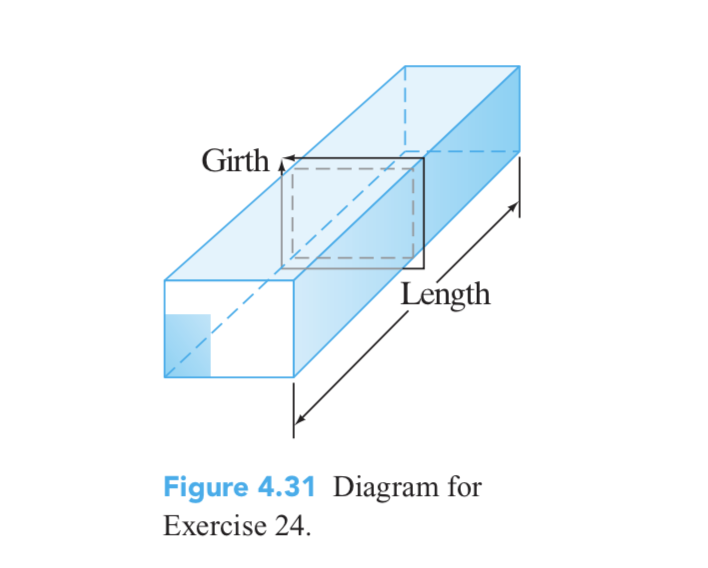
\includegraphics[scale=0.6]{assets/12_2.jpg}
  \end{figure}
\clearpage

\begin{problem}[Colley 4.3.26]
An industrious farmer is designing a silo to hold her
$900\pi$ $ft^3$ supply of grain. The silo is to be cylindrical in shape with a hemispherical roof. (See Figure 4.32) Suppose that it costs five times as much (per square foot of sheet metal used) to fashion the roof of the silo as it does to make the circular floor and twice as much to make the cylindrical walls as the floor. If you were to act as consultant for this project, what dimensions would you recommend so that the total cost would be a minimum? On what do you base your recommendation? (Assume that the entire silo can be filled with grain.)
\end{problem}
  \begin{figure}[ht]
    \centering
    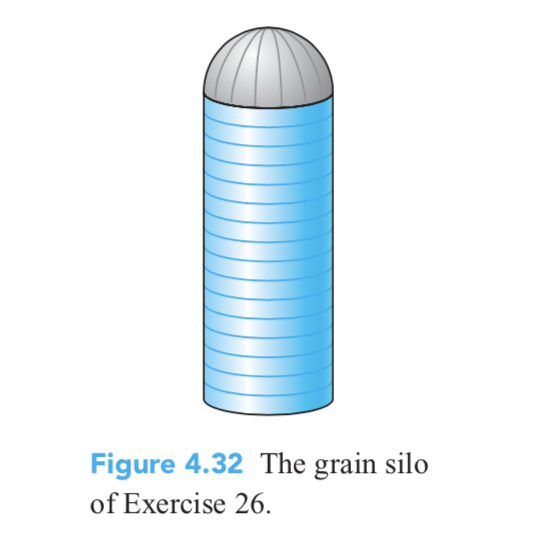
\includegraphics[scale=0.6]{assets/12_1.png}
  \end{figure}
\clearpage
\end{document}